\section{Galimi kodo skirstymo į paketus šablonai}
Diskusijose, kaip reikėtų skirstyti programini kodą, paprastai akcentuojami du šablonai - pagal \textit{techninį sluoksnį}, todo: šaltiniai, nurodantys skirstymo būdus
kur kiekvienam funkcionalumui arba kompiuterinės sistemos sluoksniui yra sukuriamas paketas,
grupuojant skirtingų dalykinių sričių esybes, arba pagal \textit{dalykinės srities esybes}, kur vienos esybės kodas, dalykinės srities
esybės funkcionalumas skirtingose programiniuose sluoksniuose yra patalpintas viename pakete.
Tačiau šie du šablonai yra gan platūs ir galėtų būti išskaidyti į daugiau smulkesnių ir tiksliau aprašytų šablonų.
Taip pat, minėtuose šablonuose, būdai kaip ir kodėl skaidyti programinį kodą parinkti akecentuojant tai, kaip programinį
kodą supranta žmonės, dirbantys prie to kodo.
Nuspresti, kaip žmones supranta programinį kodą yra gan sudėtingas ir subjektyvus procesas, todėl aprašant šablonus, kodo skirstymui
geriau akcentuoti, kaip sugrupuoti paketai bendrauja tarpusavyje ir skirstyti juos pagal klasių naudojimo atvejus ir priklausomybes.
Taip kodo grupavimo metodai yra labiau artimi Martino aprašytiems principams.
Šablonus kaip grupuoti kodą, akcentuojant klasių naudojimo atvejus ir priklausomybes nagrinėja Martin Sandin savo
straipsnyje \textit{Four Strategies for Organizing Code}.
Šis straipsnis idomus tuo, kad autorius nesiplečia į du dažniausiai sutinkamus šablonus - grupuoti pagal techninį sluoksni arba dalykinės srities esybes,
o aprašo keturis grupavimo būdus arba šablonus, kurie, nors ir įkvėpti minėtų dviejų budų, yra gan unikalūs ir labiau techniškai apibrėžti.


\subsection{Pagal komponentą}
Organizavimas pagal komponentus sumažina sistemos sudėtingumą, pabrėždamas išorinę ir vidinę kodo vienetų darną.
Išorinė darna reiškia, kad paketas turi minimalią sąsają \angl{interface}, kuri atskleidžia tik konceptus (metodus arba duomenų tipus),
kurie yra glaudžiai susiję su komponento teikiama paslauga.
Vidinė darna reiškia, kad pakuotėje esantis kodas yra stipriai susijęs tarpusavyje ir susijęs su teikiama paslauga.

Kodas yra grupuojamas į mažus paketus, turinčius vieną, aiškiai apibrėžtą funkcionalumą ar tikslą, aprašant abstrakciją, kokie paketo elementai
yra pasiekiami iš išorės ir kaip jie naudojami.
Taip sukuriamas kodas, kuris yra lengviau suprantamas.
Tokią kodo grupavimo tvarką sunku palaikyti, tačiau jos rezultatas - kodas, kuris yra lengviau suprantamas, lengviau pagerinamas, lengviau testuojamas
ir, dėl aiškiai aprašytų sąsajų, lengviau pernaudojamas.

\begin{figure}[H]
    \centering
    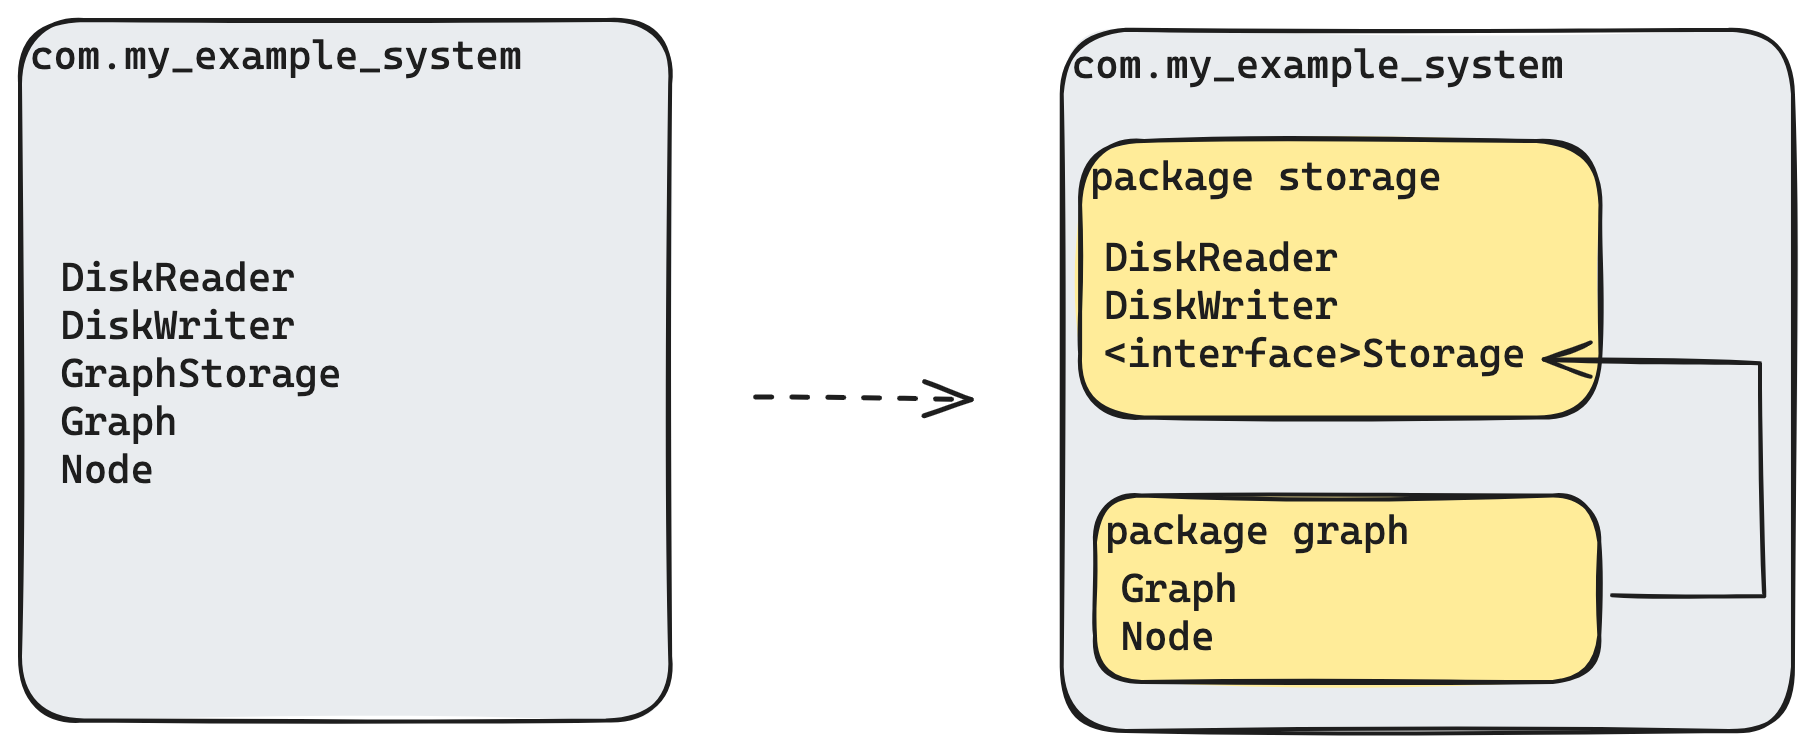
\includegraphics[scale=0.2]{img/component_packaging}
    \caption{Sistemos sugrupuotos pagal komponentą pavyzdys}
    \label{img:component_packaging}
\end{figure}


\subsection{Pagal techninį sluoksnį}
Laikantis skirstymo pagal techninį sluoksnį, kiekvienam funkcionalumui arba kompiuterinės sistemos sluoksniui yra sukuriamas paketas,
kuris savyje grupuoja skirtingas dalykinės srities esybes. Pavyzdžiui, visos sąsajos darbui su duomenų baze guli viename pakete, sąsajos
su verslo logikos transformacijomis kitame, o duomenų vaizdavimo klientui logika trečiame pakete.
Šis paketų skirstymo metodas yra labai paplitęs, ypač tarp senesnių kompiuterinių sistemų. Jį paprasta įgyvendinti,
metode paprasta pavadinti paketus, aišku, į kuriuos paketus priskirti klases. Nors tokią kodo struktūrą lengva įgyvendinti ir palaikyti sistemoje,
ji turi nemažai trūkumų. Šis metodas nepalengvina sistemos plėtros valdymo - augant sistemai paprastai daugėja dalykinės srities esybių,
o ne funkcinių sluoksnių, todėl esamų paketų skaičius beveik nesikeičia, bet klasių kiekis pakete vis auga, tai daro neigiamą įtaką navigacijai
paketo viduje. Skirstant paketus pagal funkciją taip pat nėra gerinamas informacijos slėpimas (inkapsuliacija) - kiekvienas paketas savyje
talpina skirtingų dalykinės srities esybių kodą, tai sudaro salygas per klaidą užmegzti komunikaciją tarp komponentų, kurie neturėtų būti susiję.
Taip pat, skirstant tokiu būdu, sąsajos yra stipresnės tarp loginių komponentų, pasiskirsčiusių per sluoksnius, nei tarp vieno sluoksnio esybių.
Tokiu atveju pokyčių pristatymas pasidaro sudėtingas, nes reikalinga keisti ne vieną sluoksnį.
Tačiau šis metodas turi ne tik trūkumus - vienas iš jo privalumų - ganėtinai aiškiai nusakoma bendra sistemos architektūra, programiniai sluoksniai.
Deja, netvarkinga sistemos būsena eliminuoja ši privalumą.

\subsection{Pagal tipą}
Kodo organizavimas pagal tipą įprastai nėra griežtai apibrėžtas - klasės grupuojamos pagal vartotojo sumanytą tipą, neteikiant svarbos
klasių sąryšiams ar loginėms esybėms. Taip skirstant klases, į paketus galėtų būti grupuojamos esybių, išimčių ar serviso klasės. Šis skirstymo būdas
neteikia prioriteto nei skirstymui pagal techninius sluoksnius, nei pagal dalykinės srities esybes. Jį ganėtinai nesudėtinga įgyvendinti,
tačiau šis metodas yra netvarkingas bei turi trūkumų. Taip suskirstytas kodas sunkiai skaitomas, nes nėra aišku, pagal kokią tvarką
ieškoti konkrečios klasės ar kaip priskirti esamiems paketams netinkamas klases. Taip pat toks skirstymo būdas visiškai nepadeda spręsti
klasių sąsajų problemų, kadangi neapgalvotai išskirstyti sluoksniai gali būti glaudžiai susiję.

\subsection{Pagal funkciją}
Šis skirstymo būdas dalinai panašus į skirstymą pagal komponentą, tačiau yra mažiau griežtas ir
prioritetas teikiamas ne vidinei darnai ir glaudžiai grupuojamų
komponentų sąsajai, o išorinei darnai. Tokio skirstymo būdo paketuose dažniausiai grupuojamos tos pačios sąsajos implementacijos,
parenkamos siekiant pabrėžti išorinę darną ir sugrupuoti klases, teikiančias panašias funkcijas. Toks skirstymas patogus, pavyzdžiui,
techninių bibliotekų vartotojams, kadangi galima lengvai surasti bibliotekos teikiamas funkcijas. Tokią kodo grupavimo tvarką sunku palaikyti,
nes reikia gerai apgalvoti skirstymo strategiją, kad ji būtų prasminga ir patogi naudoti.

